\chapter{Классификация существующих решений}

	Данный раздел посвящен разбору методов сжатия и их классификации.

    \section{Существующие решения}
    
    \subsection{RLE}
    
    RLE (run lenght ecoding) --- алгоритм сжатия данных, суть которого состоит в  замене цепочек или серий
    повторяющихся байтов или их последовательностей на один кодирующий байт и счетчик числа их повторений. \cite{RLE}
    
    \begin{figure}[h!]
    	\centering
    	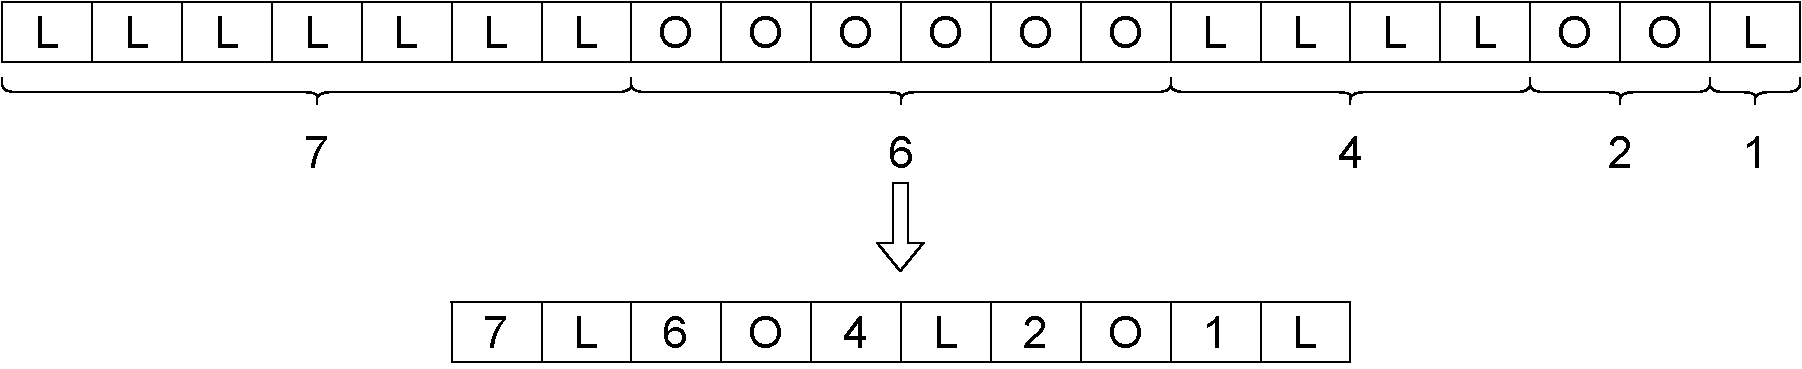
\includegraphics[width=\textwidth,height=7cm,keepaspectratio]{rle01.pdf}
    	\caption{Пример работы алгоритма RLE.} \label{fig:rle01}
    \end{figure}

	Недостатком метода RLE является достаточно низкая степень сжатия или
	стоимость кодирования файлов с малым числом серий и, что еще хуже --- с
	малым числом повторяющихся байтов в сериях. К положительным сторонам
	алгоритма, пожалуй, можно отнести только то, что он не требует
	дополнительной памяти при работе, и быстро выполняется.
    
    
    \subsection{Метод Хаффмана}
    
    Метод Хаффмана (носит имя создателя David Albert Huffman) --- жадный алгоритм оптимального префиксного кодировния алфавита. Методика гарантирует однозначное построение кода с наименьшим для данного распределения вероятностей средним числом символов на букву.\cite{haff}
    
    Метод разделен на два этапа.
    \begin{enumerate}
    	\item Построение оптимального кодового дерева.
    	\item Построение отображения код-символ на основе построенного дерева.
    \end{enumerate}

	 \begin{figure}[h!]
		\centering
		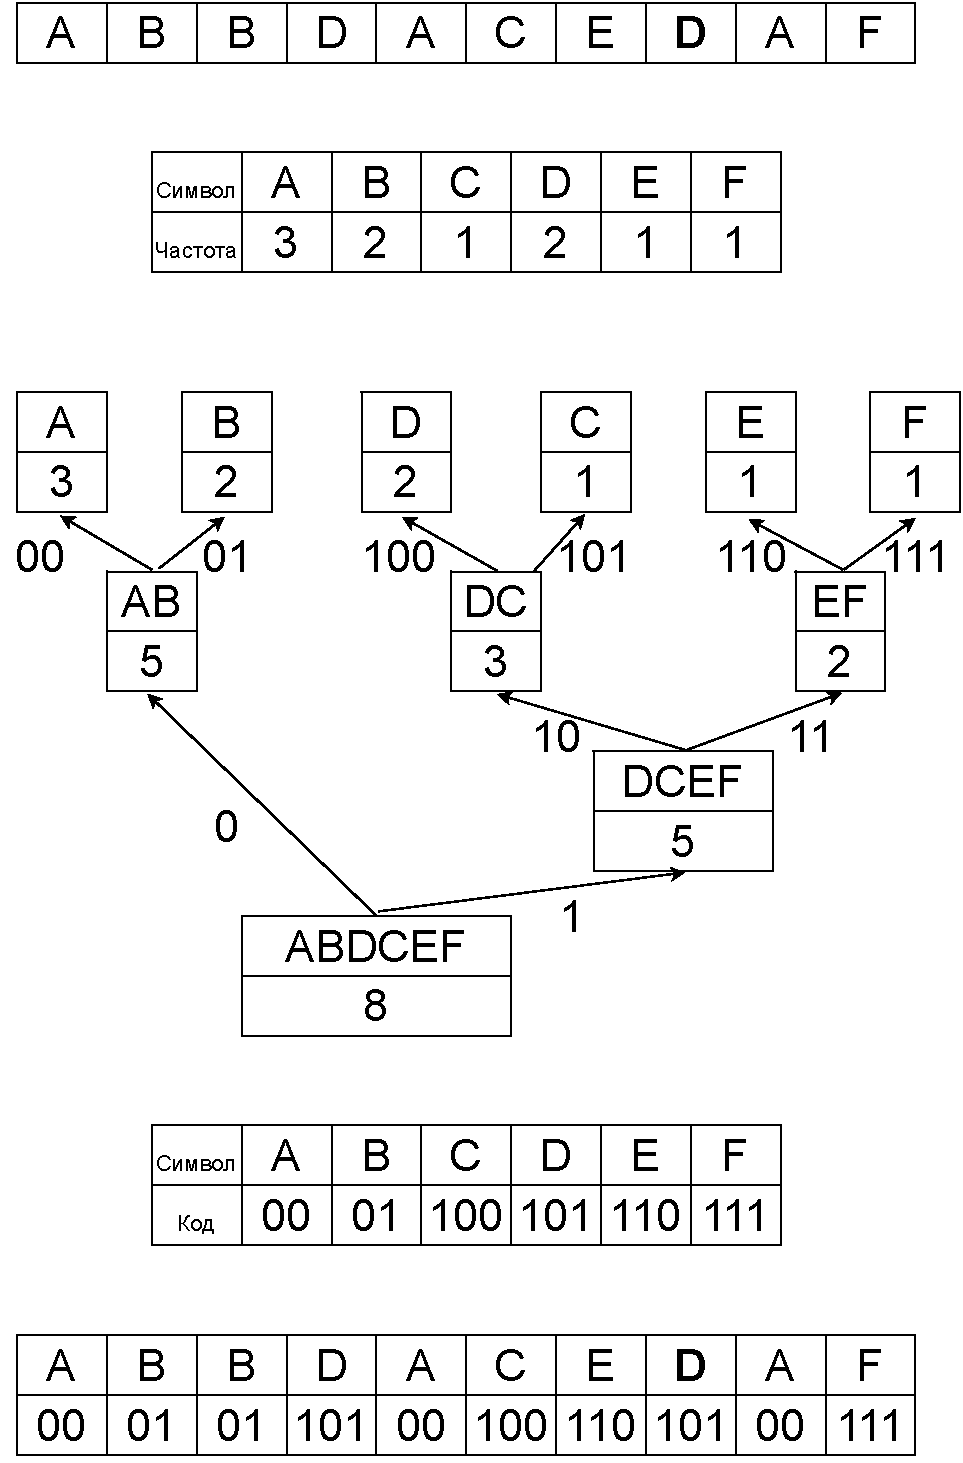
\includegraphics[width=\textwidth,height=15cm,keepaspectratio]{haff01.pdf}
		\caption{Пример работы метода Хаффмана.} \label{fig:haff01}
	\end{figure}
	
\newpage
	Применительно к сжатию изображений в основе такого метода лежит учет частоты появления одинаковых байт в изображении. При этом пикселам
исходного изображения, которые встречаются большее число раз,
сопоставляется код меньшей длины, а встречающимся редко --- код большей
длины (т.е. формируется префиксный код переменной длины). Для сбора
статистики требуется два прохода по файлу --- один для просмотра и сбора
статистической информации, второй ---  для кодирования. \cite{haff2}

При использовании такого метода требуется запись в файл и таблицы
соответствия кодируемых пикселов и кодирующих цепочек. Такое кодирование
применяется в качестве последнего этапа архивации в JPEG. Методы Хаффмана
дают достаточно высокую скорость и умеренно хорошее качество сжатия.

	Основным существенным недостатком этого метода кодирования является то, что он кодирует символы с помощью целого количества бит, что снижает степень сжатия и сводит на нет точное предсказание вероятностей, которое дают некоторые отличные современные алгоритмы моделирования. \cite{haff2}
    
    \subsection{LZW}
    
    LZW (Lempel Ziv Welch) --- алгоритм сжатия данных созданый  Авраамом Лемпелем (Abraham Lempel), Яаковом Зивом (Jacob Ziv) и Терри Велчем (Terry Welch). 
    
    %Данный алгоритм можно описать следующей последовательностю шагов.
    %\begin{enumerate}
    	%\item Инициализация словаря всеми возможными односимвольными фразами. Инициализация входной фразы первым символом сообщения.
    	%\item Если КОНЕЦ СООБЩЕНИЯ, то выдать код для W и завершить алгоритм.
    	%\item Считать очередной символ K из кодируемого сообщения.
    	%\item Если фраза WK уже есть в словаре, то присвоить входной фразе W значение WK и перейти к Шагу 2.
    %	\item Иначе выдать код W, добавить WK в словарь, присвоить входной фразе W значение K и перейти к Шагу 2.
    %\end{enumerate}
    
    Суть данного алгоритма состоит в следующем: упаковщик постоянно
хранит некоторое количество последних обработанных символов в буфере. По
мере обработки входного потока вновь поступившие символы попадают в
конец буфера, сдвигая предшествующие символы и вытесняя самые старые.
Размеры этого буфера, называемого также скользящим словарем, варьируются
в разных реализациях кодирующих систем. Затем, после построения 
таблиц, выделяют (путем поиска в словаре) самую длинную начальную
подстроку входного потока, совпадающую с одной из подстрок в словаре, и
выдают на выход пару (length, distance), где length --- длина найденной в словаре
подстроки, а distance --- расстояние от нее до входной подстроки (то есть
фактически индекс подстроки в буфере, вычтенный из его размера). Если такая
подстрока не найдена, в выходной поток просто копируется очередной символ
входного потока. \cite{LZW}

Существует довольно большое семейство LZ-подобных алгоритмов,
различающихся, например, методом поиска повторяющихся цепочек. Один из
достаточно простых вариантов этого алгоритма, например, предполагает, что во
входном потоке идет либо пара <счетчик, смещение относительно текущей
позиции>, либо просто <счетчик> 'пропускаемых' байт и сами значения
байтов.

При разархивации для пары <счетчик, смещение> копируются <счетчик>
байт из выходного массива, полученного в результате разархивации, на
<смещение> байт раньше, а <счетчик> (т.е. число равное счетчику) значений
"пропускаемых" байт просто копируются в выходной массив из входного
потока.

Данный алгоритм является несимметричным по времени, поскольку
требует полного перебора буфера при поиске одинаковых подстрок.
К достоинствам LZ можно отнести чрезвычайную простоту алгоритма
декомпрессии.
    
    %\subsection{Арифметическое сжатие}
    
    
    \subsection{JPEG}
    
    JPEG (Joint Photographic Experts Group) --- формат хранения фотографических изображений, отличающийся хорошим качеством восстановленного изображения. Процесс сжатия изображения JPEG достаточно сложен и часто для достижения приемлемой производительности требует специальной аппаратуры. Схема процедуры сжатия изображений по стандарту JPEG приведена на ниже. \cite{JPEG1}
    
     \begin{figure}[h!]
    	\centering
    	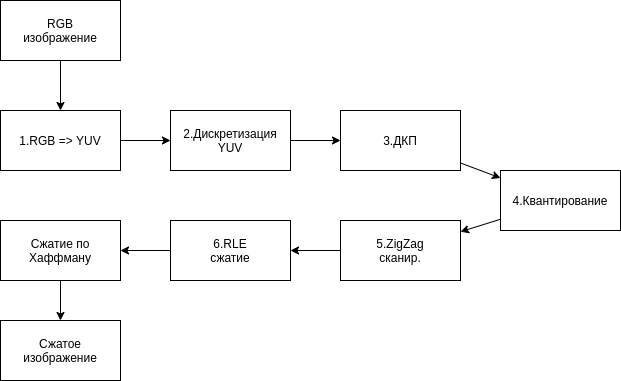
\includegraphics[width=\textwidth,height=8cm,keepaspectratio]{jpegdi.png}
    	\caption{Основные этапы процедура сжатия по стандарту JPEG.} \label{fig:jpegdi}
    \end{figure}
    
    1. RGB => YUV.
    
    Преобразование RGB  в YUV(Y-компонента --- яркость, две остальные --- голубая и красная компоненты). Цветное изображение в RGB представляется в виде
     \begin{equation}
      X_C = a_{1}X_R + a_{2}X_G + a_{3}X_B,
\end{equation}     
     
     где
     
      \(a_1\), \(a_2\) и \(a_3\) --- калориметрические коэффициенты.
    
    Для получения YUV используют формулу 
    \begin{equation}
    Y = \sqrt{a_{1}{X_R}^2 + a_{2}{X_G}^2 + a_{3}{X_B}^2}      
    \end{equation}
    
   
    
    \begin{equation}
    U = X_B
    \end{equation}
    
    \begin{equation}
    V = X_R.
    \end{equation}
    
    2. Дискретизация YUV.
    
    Исходное изображение разбивается на блоки, размером 8×8 пикселей. На этом этапе используется то, что яркостная и цветовая составляющие изображения хранятся отдельно. Для увеличения степени сжатия дискретизация проводится для разных составляющих с разной частотой – изображение делится по компоненте Y, а для компонент U и V цветовая информация берется через строку и через столбец. Таким образом, сразу получаем степень сжатия в два раза, а на качестве изображения это сказывается не сильно.
    
    3.ДКП.
    
    Основным этапом работы алгоритма является дискретное косинусное преобразование (ДКП), позволяющее переходить от пространственного представления изображения к спектральному. Обработка каждого блока выполняется независимо и заключается в применении к каждой рабочей матрице формулы  \cite{JPEG2}
    \begin{equation}
      F(\textit{u, v}) = \frac{1}{4} C(\textit{u}) C(\textit{v}) \left[ { 
		\displaystyle\sum_{x=0}^{7}   \displaystyle\sum_{y=0}^{7}   \textit{f} (x, y) 
		\cos \frac{(2x + 1) \textit{u} \pi }{16} \cos \frac{(2x + 1) \textit{v} \pi }{16}
 	} \right], 
    \end{equation}
  
 	где 
 	\begin{equation}
 	C(z) = \begin{cases}
 		\frac{1}{\sqrt{2}},  & \mbox{если } z = 0 \\
 		1, &  \mbox{иначе.}
 	\end{cases} 
 	\end{equation}
 	
 
 	В получившейся матрице коэффициентов низкочастотные компоненты расположены ближе к левому верхнему углу, а высокочастотные --- справа и внизу. Для восстановления сжатого изображения гораздо более важны значения низких частот, чем значения высоких, потому что медленные изменения цвета в изображении более замены, чем быстрые.

	4. Квантование.
	
	Именно на этом этапе происходит самая значительная потеря информации. Квантование представляет собой деление каждого полученного после ДКП блока коэффициентов на матрицу квантования поэлементно. Для каждой компоненты матрица квантования своя. Значение коэффициентов этой матрицы определяет степень сжатия изображения. Поскольку для U и V компонентов квантование может быть более грубым, чем для Y компонента, на последнем этапе процесса сжатие U и V компонентов происходит в большей степени. После квантования большинство значений в блоке становятся нулями, сохранятся только небольшое количество наиболее значимых коэффициентов, к тому же эти значения относительно невелики. Квантование также обеспечивает возможность последующего эффективного сжатия данных при помощи любого способа сжатия без потерь.
	
	5. ZigZag сканирование.
	
	Для этого блок 8×8 обходим при помощи зигзаг-сканирования, все коэффициенты вытягиваются в цепочку. В начале этой цепочки находятся коэффициенты, соответствующие низким частотам, а в конце --- высоким. 
	
	6. RLE (рассмотрен выше). 
	
	7. Метод Хаффмана (рассмотрен выше).
	
	
	JPEG --- один из самых популярных алгоритмов сжатия. Он обеспечивает высокую
	эффективность сжатия при приемлемом уровне потерь. JPEG применяется, в основном,
	к фотореалистичным изображениям. Основной плюс этого алгоритма – это высокие коэффициенты сжатия изображений. К минусам можно отнести высокую вычислительную сложность и специфические искажения – эффект Гиббса. Этот эффект проявляется
	в том, что линии JPEG изображений с четкими контурами начинают заметно «дрожать». Так, например, если изображение содержит какие-либо подписи, то подобный
	эффект может возникнуть вокруг символов.
	
    
    \subsection{Фрактальное сжатие}
    
    Различные методы сжатия изображений основываются на устранении тех или иных форм избыточности, в частности, фрактальные методы рассматривают самоподобие как источник избыточности. Считается, что самоподобие является свойством почти всех природных объектов и их изображений, и, следовательно, устранение этой формы избыточности может значительно уменьшить объем данных, необходимых для описания природного объекта или его изображения.\cite{frac}
    
    Фрактал --- это структура, выделенная при анализе изображения и обладающая схожей формой независимо от ее размеров. Например, в изображении кроны дерева фрактал --- изображение листа. Фрактальное сжатие изображений основано на гипотезе, согласно которой в любом изображении можно обнаружить локальное самоподобие
    различных его частей.\cite{91}
    
    При фрактальном сжатии изображение представляется в более компактной форме --- с помощью коэффициентов системы итерируемых функций (IFS). IFS представляет
    собой набор трехмерных аффинных преобразований, переводящих одно изображение в
    другое. Преобразованию подвергаются точки в трехмерном пространстве (x-координата, у-координата, яркость). Фактически фрактальная компрессия – это поиск
    самоподобных областей в изображении и определение для них параметров аффинных
    преобразований. \cite{fr}
    

	Наиболее распространённым примером фрактального изображения,
сгенерированного с помощью IFS является изображение папоротника, использованное для создания данного изображения (Рисунок \ref{fig:pap}),  состоит из 4-х
аффинных преобразований. Каждое преобразование кодируется считанными
байтами, хотя исходное изображение может быть любого размера. Таким
образом, можно заключить, что фрактальная компрессия --– это поиск
самоподобных областей и определение для них параметров аффинных
преобразований.    
    
     \begin{figure}[h!]
    	\centering
    	
\includegraphics[width=\textwidth,height=7cm,keepaspectratio]{pap.png}
    	\caption{Изображение папоротника, сгенерированного с помощью IFS.} \label{fig:pap}
    \end{figure}
    %\subsection{JPEG2000}
    
\newpage    
    
    \section{Классификация методов сжатия изображений}
    
    %\subsection{Классифицируется по степени сохранности информации до и после сжатия.}
    
    Все способы сжатия можно разделить на две категории: обратимое (без потерь) и необратимое (с потерями) сжатие.
%Обратимое сжатие, или сжатие без потерь, приводит к снижению объема выходного потока информации без изменения его информативности, т. е. без потери информационной структуры.
%Другими словами, после выполнения операции декодирования получается поток, в точности совпадающий с потоком данных источника. Обратимое сжатие обычно используется при кодировании текстовой информации.
    
    \textbf{Методы сжатия без потерь}
    
    Во время сжатия и распаковки информация не теряется. Она в основном используется для архивирования изображений. Ее особенностью является отсутствие потери информации, но степень сжатия ограничена.
    
    \begin{itemize}
    		\item упаковка пикселей (RLE);
    		
    		%Алгоритмы данного семейства выделяют в потоке данных (в изображении) группы однородных элементов (байтов, пикселей) и выполняет замену этих групп парой чисел, одно из которых определяет значения повторяющихся элементов (цветовые характеристики байтов, пикселей), а другое – количество элементов в этой группе. В том случае, если в изображении в достаточном количестве присутствуют группы однородных элементов, происходит существенное сокращение объёмов информации. К сожаленью, в компьютерной графике подобные алгоритмы эффективно работают при малой цветности изображений - до 256 цветов (т.е. до 8 бит/пиксель).Эти алгоритмы в англоязычной литературе называются RLEалгоритмами (Run Length Encoding). 
    		
    		%\item групповое кодирование;
    		\item методы, базирующиеся на словаре (LZW);
    		
    		
    		
    		\item методы, базирующиеся на кодировании строк бит переменной длины (Метод Хаффмана).
    \end{itemize}
    
    
    \textbf{Методы сжатия с потерями}
    
    Уничтожение части информации для получения высокой степени сжатия. Этот тип сжатия обычно используется в приложениях цифрового телевидения, передачи изображений и мультимедиа. Он характеризуется игнорированием вторичной информации, которая не чувствительна к человеческому зрению Коэффициент сжатия, также известный как сжатие с потерями.
    
    %\textbf{Извлечение функций}
    \begin{itemize}
    		\item JPEG-сжатие;
    		%\item волновое сжатие (вейвлет-сжатие);
    		\item фрактальное сжатие.
    \end{itemize}
     
    
 	%\subsection{По методу сжатия изображения его можно разделить на четыре категории.}
 	
    
    %\textbf{Пиксельное кодирование}
    
    %Только каждый пиксель обрабатывается отдельно при кодировании. Такие как импульсная кодовая модуляция, энтропийное кодирование, кодирование по длине прогона и т. д.
    
    %\textbf{Предиктивное кодирование}
    
    %При удалении корреляции и избыточности между соседними пикселями кодируется только новая информация. Обычно используются дифференциальная импульсная кодовая модуляция.
    
    
    %\textbf{Преобразование кодирования}
    
    %Определенное преобразование применяется к данному изображению, так что большой объем информации может быть представлен с меньшим количеством данных. Обычно используемые преобразования включают в себя: дискретное преобразование Фурье (DET), дискретное косинусное преобразование (DCT) и дискретное вейвлет-преобразование (DWT).
    
   	%\textbf{Другие методы}
   	
   	%Раннее кодирование, такое как смешанное кодирование, векторное квантование, алгоритм LZW.
   	%В последние годы появилось много новых методов кодирования со сжатием, таких как алгоритмы кодирования со сжатием с использованием искусственных нейронных сетей, фрактальные, вейвлет, методы кодирования на основе объектов, алгоритмы кодирования на основе моделей Подождите.
    
    
   % Идея словарных методов:
    %\begin{itemize}
    %	\item рассматриваем входную последовательность как последовательность строк, содержащих произвольное количество
    	%символов;
    	%\item при кодировании заменяем строки символов на кода (индексы строк в некотором словаре);
    %	\item при декодировании осуществляется замена индексов на соответствующие им фразы словаря.
    %\end{itemize}	

    %Словарь --- это набор строк, которые предположительно будут встречаться в обрабатываемой последовательности. Индексы строк должны быть построены таким образом, чтобы в среднем их представление занимало меньше места, чем требуют замещаемые строки. За счет этого и происходит сжатие.
    
    
    
    %В основе методов неравномерного кодирования лежит идея: «если представлять часто используемые элементы короткими кодами, а редко используемые – длинными кодами, то для хранения блока данных требуется меньший объем памяти, чем если бы все элементы представлять кодами одинаковой длины». Для однозначного декодирования неравномерного кода будем считать, что никакое кодовое обозначение не совпадает с началом какого-
    %либо другого более длинного кодового обозначения (другими словами, код является префиксным).
     \newpage
    
    \begin{figure}[h!]
    	\centering
    	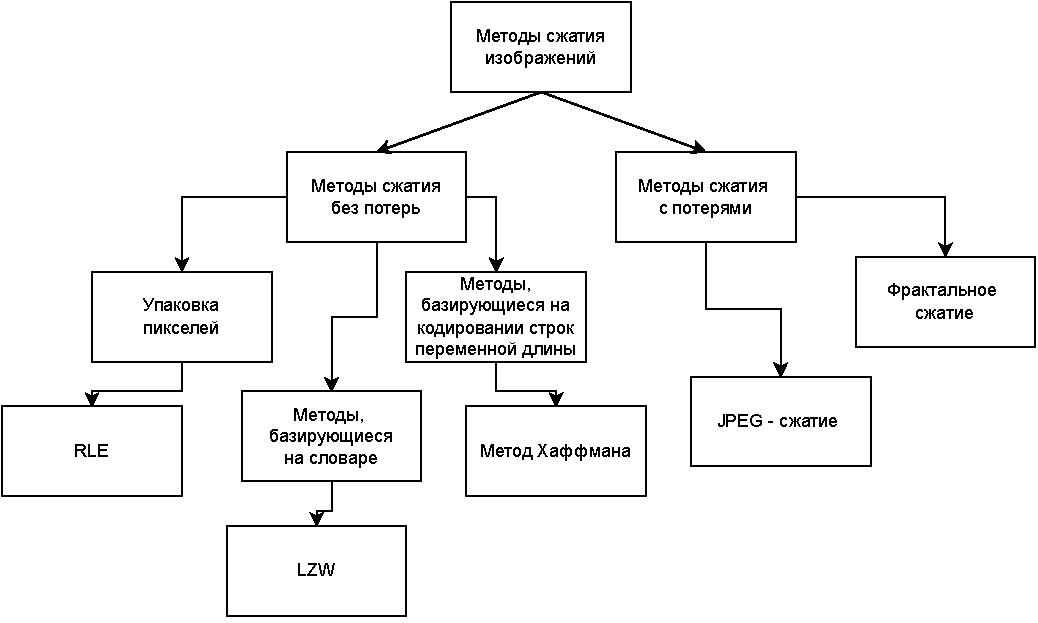
\includegraphics[width=\textwidth,height=10cm,keepaspectratio]{klassData.pdf}
    	\caption{Классификация методов сжатия изображений.} \label{fig:klassData}
    \end{figure}

    \section{Вывод}
    
    В данном разделе рассмотрены методы сжатия изображений, показаны их плюсы и минусы. А так же проведена классификация данных методов.
%Разные методы сжатия обладают разными качествами. Каждый из них имеет свои плюсы и минусы. Каждый из них имеет свою область применения. Классификация этих методов позволяет выбрать оптимальный вариант для решения конкретной задачи.